\section{Introduction}
Navigation is one of the fundamental tasks in mobile robotics. For robots with reasonable dynamics and operating speeds in indoor environments, efficient collision-free navigation is practically solved. However, introducing constraints other than ``please take the shortest path without running into anything'' is still an ongoing area of research, especially when taking the social needs of humans into account. However, the best methods and parameters for adding the constraints has not been adequately explored. 

Take the environment shown in Figure \ref{fig:intro}. The world is discretized into a grid of cells. In the original formulation \cite{matthies1988}, each cell was either occupied or free. The occupied cells are considered ``lethal'' since they would result in a collision for the robot.\footnote{This does not refer to the robot lethally injuring humans.} The extension of these Occupancy Grids is costmaps, which can have a whole range of values (represented by $f(x,y)$). If the value is greater than some limit $L$. The free cells are marked with $f(x,y)=0$. Everything in between is a ``non-lethal'' obstacle. 

What does it mean for a cell to be non-lethal? They can mark places where there might be an obstacle, but more interestingly they can denote locations where it is undesirable to be for one reason or another, but does \emph{not} result in a collision. Raising the value of the cells makes it less likely for the robot to travel into those cells. But how much less likely? Under what conditions? The answer is, it depends. 

In Figure \ref{fig:intro}, there are two possible paths that do not enter any lethal cells.  The robot could either take the shortest path, or it could take a longer path but avoid the non-lethal obstacle. The actual path that is taken depends on two separate components. The first is the costmap itself, which can be statically generated or created from sensor data. The costmap actually defines the values for all of the cells. As a separate entity, there is the path planning algorithm itself, which calculates the path with the least total cost. The standard algorithms such as Dijikstra's and A* can be used on the costmap. To optimize for path length (and thus avoid wayward paths that avoid every hint of an obstacle), wavefront planners are often used, which add a constant value to each cell traversed to create a gradient from start to finish\cite{choset:principles}. The interplay between the values in the costmap and the path planning constant turns out to be crucial for determining which path is optimal. 

Non-lethal obstacles are useful for representing general preferences/guidelines rather than hard and fast rules. Policies such as ``do not enter the kitchen unless there is no other path'' and ``leave some room between you and the wall when you can'' can easily be implemented as non-lethal obstacles. One of the most frequently used scenarios for such obstacles is for representing people's desired behavior in relation to the location of the robot. As \citet{kirby:companion} observed, ``Human social conventions are tendencies, rather than strict rules,'' arguing that the binary costmap (occupied/unoccupied) is inadequate for representing human constraints. For concepts such as a person's personal space, non-lethal obstacles have proven useful, although what is the ``best'' path is not clear. 

The existence of such obstacles does not necessitate that the robot does not break the guidelines. The robot can still enter a person's personal space, or enter the kitchen, if there are no better options. Creating paths from non-lethal costmaps gives roboticists a way to rank multiple different legal options for some metric based on the desired behavior. 

However, creating the desired behavior is often more difficult than one would think. While previous researchers have all tuned their parameters to create working configurations, there exists no general guide for how to tune the parameters to change the robot behavior. Furthermore, as our exploration of this space shows, the behavior is not always readily intuitive. 

%This paper aims to explore the space of these paths through non-lethal costmaps. 

%Occupancy Grids have proven useful over the years because their volumetric representation allows for unstructured data from heterogeneous sources. These binary values are used to construct a graph with which planning can be done using Dijkstra's algorithm or any of its variants. However, such Occupancy Grids cannot represent non-lethal obstacles. The more advanced representation of costmaps can take any arbitrary number of values, however, in practice, such grids often devolve into the highest values representing occupied, the lowest representing unoccupied, and everything in between is largely untouched. 

\begin{figure}
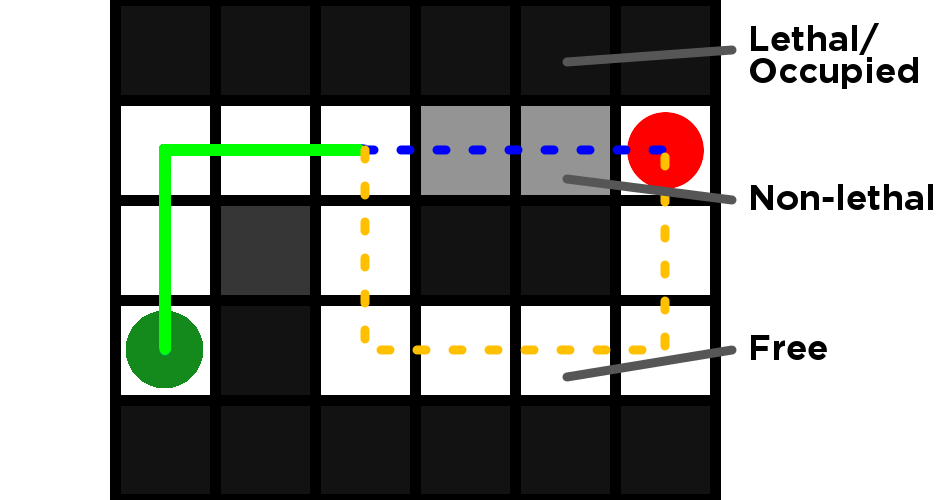
\includegraphics[width=\columnwidth]{graphix/Intro.png}
\caption{Simple Costmap with Non-lethal Obstacles - There are two possible paths for the robot. The path in blue is the shortest possible path, but enters the non-lethal obstacle. The yellow path is longer but avoids the obstacle. Which path is optimal and which is the path less traveled depends on how the costmap \emph{and} the path planner are configured. }
\label{fig:intro}
\end{figure}


